\documentclass[11pt]{article}
\usepackage[pdftex]{graphicx}
\usepackage{amsmath}
\usepackage[margin=1.0in]{geometry}

\title{Physics performance of the Day 1 Near Detector}
\author{Chris Marshall (University of Rochester), for the DUNE collaboration}
\date{31 January 2021}

\begin{document}

\maketitle

\section{Introduction}
\label{sec:intro}

% Definine goal, reference vs. D1ND
This chapter examines the impact of the near detector (ND) on the sensitivity of DUNE to long-baseline neutrino oscillations. In particular, we consider the full reference near detector described in the CDR and consisting of the liquid argon TPC (ND-LAr), the magnetized high-pressure gaseous argon TPC and surrounding calorimeter (ND-GAr), and beam monitor (SAND). We also consider the ``Day 1 Near Detector'' (D1ND) consisting of ND-LAr and the temporary muon spectrometer (TMS), where the beam monitoring capability of SAND is also assumed. These individual detectors are described in detail elsewhere in the PDR.

% Long-term goals
DUNE is designed to make precision measurements of long-baseline neutrino oscillations. A primary objective articulated in the P5 strategy is observing CP violation at 5$\sigma$ for 50\% of the true values of $\delta_{CP}$. This measurement requires thousands of $\nu_{e}$ and $\bar{\nu}_{e}$ events at the Far Detector (FD), and a robust ND to constrain systematic uncertainties to a level comparable to the FD statistical uncertainty of 2-3\%. The reference ND is designed to provide this constraint by combining high-statistics measurements with a detector similar to the FD (ND-LAr) with a suite of $\nu$-Ar measurements with precision far beyond the FD (ND-GAr), off-axis measurements that directly probe energy dependence (PRISM), and beam monitoring (SAND). The reference sensitivity to CP-violation and the resolution to $\delta_{CP}$ are shown as a function of time in Figure~\ref{fig:longterm_sensitivity}. Over the first few hundred kiloton-megawatt-years (kt-MW-yrs), the sensitivity improves rapidly with exposure as statistics are accumulated in the FD, and the sensitivity is less dependent on the near detector. After several hundred kt-MW-yrs, the sensitivity becomes highly dependent on systematic uncertainties and on the performance of the ND.

\begin{figure}[h]
\centering
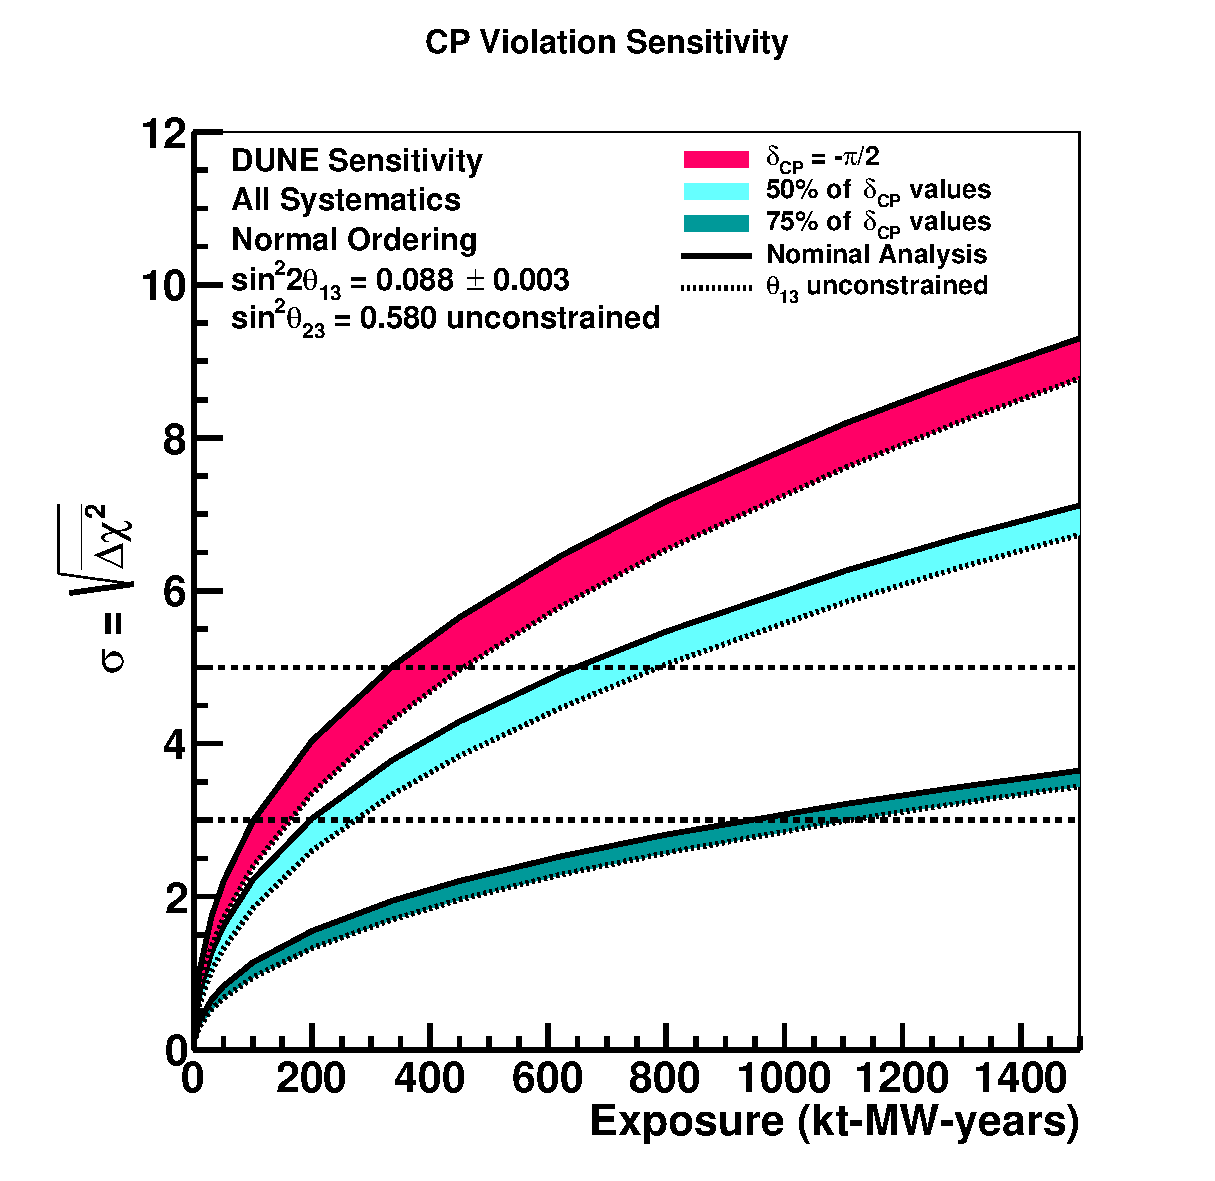
\includegraphics[width=0.45\columnwidth]{graphics/cpv_exp_varyconstr_nh_2019_v4.eps}
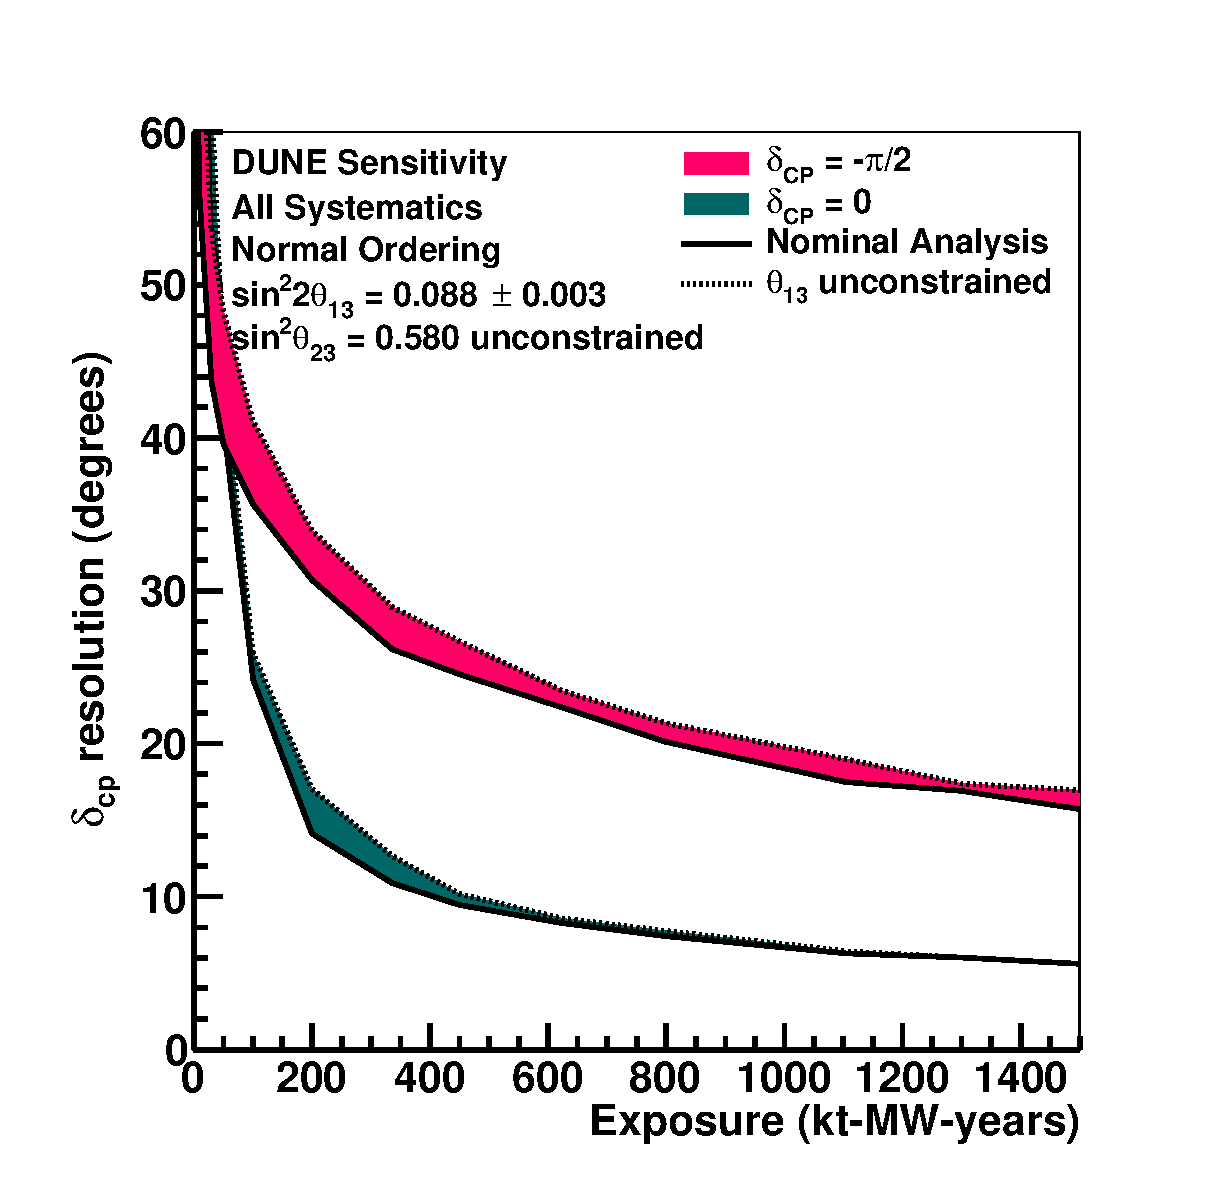
\includegraphics[width=0.45\columnwidth]{graphics/dcpres_exp_varyconstr_nh_2019_v4.eps}
\caption{The reference sensitivity to CP violation (left) and resolution on $\delta_{CP}$ (right) is shown as a function of exposure. For the initial beam intensity of 1.2 MW, the exposure is 24 (48) kt-MW-yrs per calendar year for 2 (4) FD modules; these numbers double when the beam intensity is upgraded to 2.4 MW.}
\label{fig:longterm_sensitivity}
\end{figure}

% Short-term goals, define the metrics
At the initial design intensity of 1.2 MW, the rate of $\nu_{e}$ charged-current (CC) interactions in the FD is $\sim 100$ per 10 kt module per year of operation if the mass ordering is normal and $\delta_{CP} = -\pi / 2$. Depending on the staging scenario, it will take 4-7 years to accumulate the thousands of FD events required to make precision measurements. However, it is nonetheless possible for DUNE to make interesting and impactful neutrino oscillation measurements with just hundreds of oscillated $\nu_{e}$s. In particular, with an exposure of $\sim 70$ kt-MW-yrs ($\sim 3$ years with two FD modules at 1.2 MW), DUNE can observe CP violation at $3 \sigma$ if $\delta_{CP} = -\pi / 2$. This is by no means the only measurement that can be made with three years of data; DUNE can also resolve the neutrino mass ordering unambiguously, and make measurements of the disappearance parameters that are competitive with existing results. We use a $5 \sigma$ observation of CP violation over 50\% of $\delta_{CP}$ values as a proxy for the broad long-term physics program of DUNE, and a $3 \sigma$ observation of maximal CP violation as a proxy for the broader short-term physics program. We do this because CP violation is the highest profile measurement, it is relatively simple to evaluate, it encapsulates many of the same effects that are relevant for other measurements, and it simplifies an otherwise very complicated discussion.

% In-model and out-of-model effects, mock data
Systematic uncertainties due to the modeling of the neutrino flux, neutrino-argon interaction cross sections, and detector reconstruction effects are included in the sensitivities shown in Figure~\ref{fig:longterm_sensitivity}, and are described in detail in Ref.~\cite{lblpaper}. Cross section uncertainties in particular are challenging to parameterize because they impact not only the rate of CC neutrino interactions, but also the relationship between neutrino energy and detector observables in a highly nontrivial way. These uncertainties are typically evaluated within the framework of a particular interaction model, in this case GENIE. While our treatment goes well beyond the default uncertainties included within GENIE, there may nonetheless be out-of-model effects that are not encapsulated, and it is critical to ensure that the near detector system is capable of resolving such effects. One such out-of-model effect is obtained by generating ``mock data'' based on the NuWro model, and fitting this ``data'' with our nominal model. This fit yields a bias in $\delta_{CP}$, which can be added as an additional systematic uncertainty in quadrature to produce a modified sensitivity. The bias is only partially resolved with the D1ND, but is largely eliminated by the addition of ND-GAr as described in Section~\ref{sec:ndgar}. This additional bias significantly worsens DUNE's sensitivity to CPV for 50\% of $\delta_{CP}$ values, as shown in the left panel of Fig.~\ref{fig:nuwro_sens}. In particular the P5 goal of a $5 \sigma$ observation is not achieved. However, for the short-term goal of observing CPV for maximal $\delta_{CP}$, the additional uncertainty is small compared to the statistical magnitude of the effect of CPV, and the Day 1 Near Detector system of ND-LAr and TMS is sufficient for a $3 \sigma$ observation with a minimal delay, as can be seen in the right panel of Fig.~\ref{fig:nuwro_sens}.

\begin{figure}[h]
\centering
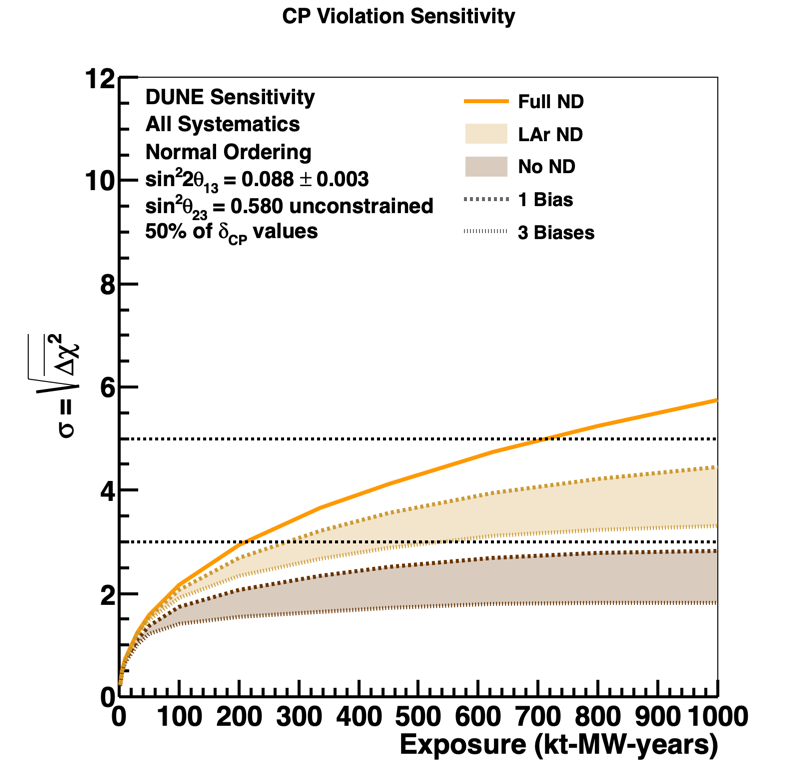
\includegraphics[width=0.45\columnwidth]{graphics/cpv_exp_nuwrobias_nd_50pc_2019_v4.png}
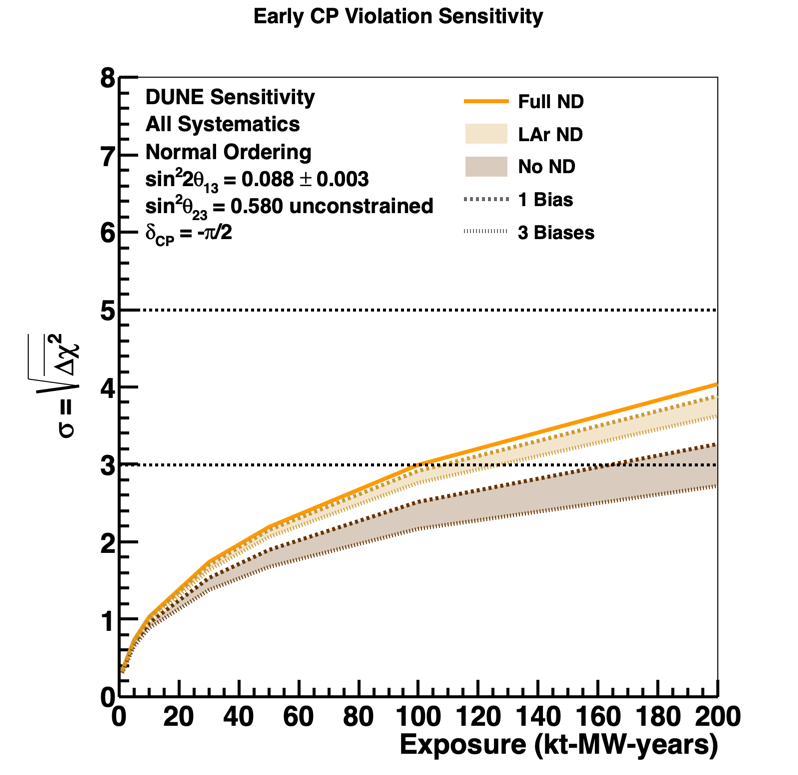
\includegraphics[width=0.45\columnwidth]{graphics/cpv_exp_nuwrobias_ndearly_max_2019_v4.png}
\caption{The sensitivity to CP violation is shown as a function of exposure in the case of the full reference ND, the Day 1 ND, and no ND or only a very limited ND. The ND configuration affects the additional uncertainty due to modeling bias. The effect is large in the case of 50\% of $\delta_{CP}$ values and long exposure (left) but modest in the case of maximal $\delta_{CP}$ and shorter exposure (right).}
\label{fig:nuwro_sens}
\end{figure}

% conclusions up front
Based on the result shown in Fig.~\ref{fig:nuwro_sens}, it is clear that the reference ND is required to achieve the long-term precision goals of DUNE, including the P5 goal of observing CP violation at $5 \sigma$ significance for 50\% of the true values of $\delta_{CP}$. This study also provides confidence that a capable near is required to enable impactful physics results to be published in the first several years of DUNE running, and that the D1ND as described in the PDR satisfies these requirements and enables a $3 \sigma$ observation of maximal CP violation. Ideally, this study would be repeated for every possible alternate interaction model to show exhaustively that these conclusions are robust and do not depend on the details of this particular NuWro model. Given our current understanding of neutrino interactions this is clearly not possible. We note in Section~\ref{sec:conclusions} why this mock data set is representative of the magnitude of potential biases, and how the PRISM technique guards against more general modeling deficiencies.

\section{Probing out-of-model effects}
\label{sec:mockdata}

An out-of-model effect is anything that modifies the reconstructed spectra in the ND or FD that cannot be obtained by shifting a parameter of the reference model. Out-of-model effects could in principle originate from any source of uncertainty, including flux, cross sections, and detector reconstruction. While it is possible and in some cases instructive to construct mock data samples with alternate fluxes or detector models, we focus on cross section effects because the neutrino interaction predictiion is the most complicated aspect of the simulation. The measured event distributions as a function of reconstructed neutrino energy are sensitive to the interaction model in highly nontrivial ways. Because the detector response varies as a function of momentum and is different for different particle species, any modification of the final state kinematics can impact the oscillation fit. Furthermore, numerous recent neutrino cross section measurements have shown large deviations from model predictions that are not described by uncertainties in the models themselves.
 
% NuWro mock data
Mock data is used to study the impact of an out-of-model effect in the cross section prediction. The mock data must be produced with a plausible alternative cross section model, and one which cannot be obtained by varying any combination of parameters within the default model. For example, creating a mock data sample by starting with the nominal model and changing the value of the cross section parameter $M_{A}^{RES}$ would not suffice, because the fit could exactly accomodate the mock data by shifting that parameter. Instead, we use an entirely different neutrino interaction generator, NuWro, to produce the mock data sample.

% How NuWro and GENIE are different off the top of CMM's head -- experts should check this
Like GENIE, NuWro is a generator that nucleon-level cross sections in various neutrino interaction channels, a description of the nuclear initial state, and nuclear final-state interactions. The nucleon-level cross sections for quasielastic scattering and resonant pion production are identical. Both models include an implementation of the two-body current contribution to quasielastic scattering (often called 2p2h or meson exchange current), but the details are different. Above the $\Delta(1232)$ resonance, the generators differ significantly. GENIE uses the KNO scaling model to predict the hadronic final state for invariant masses between 1.7 and 2.3 GeV, the PYTHIA model above $W = 3$~GeV, and the AGKY model -- a custom blend of AGKY and PYTHIA -- in between. NuWro uses PYTHIA for all inelastic events above the resonance. Neither prescription is especially well-motivated theoretically, and this region of phase space is poorly constrained by existing data. One reason for this is that many previous and current experiments like MiniBooNE and T2K operate in an energy regime where the contribution from deep inelastic scattering is very small. GENIE and NuWro also differ in their description of the nuclear initial state, and use different models to simulate final-state interactions. Neither GENIE nor NuWro perfectly describes existing data, and discrepancies between their predictions and measured cross sections are comparable in magnitude. NuWro is therefore an excellent candidate to use as mock data to study out-of-model effects; it is a plausible alternate model that differs from the nominal model in several important ways. Some of the differences (for example hadronization) are in areas where uncertainties are difficult to implement because the underlying processes are not readily reweightable.

% Why we don't run from scratch
Mechanically, repeating the entire simulation chain (neutrino event generation, particle propagation with Geant4, reconstruction) beginning with an alternative generator is not feasible for several reasons. First, the software is designed to read in events in a format specific to GENIE, and it is not straightforward to ``translate'' output from one generator format to another. Second, the computing resources required to run the Geant4 stage and the reconstruction are significant. The statistics required to do the analysis in the near detector are large (tens of millions of events), and the far detector reconstruction is relatively slow. It is preferable to produce the mock data samples by reweighting existing events. This reweighting is traditionally done as a function of one or more true kinematic quantities, for example $Q^{2}$ or $W$, and perhaps as a function of neutrino energy. The weights can be generated by simply taking a ratio between the alternate model and the nominal in whatever kinematic space. This requires running only the neutrino event generation step using the alternate model. However, this produces a result that is not representative of the alternative model, because the differences in the prediction depend on many more quantities, for example the number and momenta of final-state pions, protons, and neutrons. In principle, one could define a ratio in terms of a higher dimensional space of more kinematic quantities. But this quickly becomes impractical as the number of bins -- and hence the required simulated statistics -- grows exponentially with the number of kinematic variables.

% Reweighting -- could be expanded by Cris Vilela with more detail (in appendix?) if desired
To solve this problem, a reweighting framework was developed that uses a boosted decision tree (BDT) to determine the weights. The BDT is trained on 23 truth-level quantities, which together fully describe differences between the generators, and also map onto detector quantities like the reconstructed hadronic energy in a way that is non-degenerate. The kinematic quantities used in the training are neutrino energy, lepton energy, the angle between the lepton and neutrino, the four-momentum transfer $Q^{2}$, the hadronic invariant mass $W$, Bjorken $x$, and the inelasticity $y$. In addition, both the number and total energy of different particle species are included: protons, neutrons, $\pi^{+}$, $\pi^{-}$, $\pi^{0}$, and photons. Finally, the interaction current, neutrino helicity, and neutrino flavor are included. The BDT is designed to take the 23-dimensional truth space of GENIE and calculate a weight for each event based on those quantities such that the NuWro sample is reproduced in the 23-dimensional space when the weights are applied. The algorithm essentially enables a NuWro/GENIE ratio to be evaluated in a space sufficiently high in dimension to encapsulate all the physics differences, but with statistics of just a few million events.

% Fitting mock data
The FD mock data produced with NuWro is fit using the reference GENIE model. The mock data, nominal MC, and best fit are shown in Figure~\ref{fig:nuwro_fdfit} for each of the two neutrino flavors (muon disappearance, left, and electron appearance, right) in each of the two horn polarities (forward ``neutrino mode'', top, and reverse ``antineutrino mode'', bottom). The data points are discrepant with the reference GENIE model. The best-fit is obtained by varying flux, cross section, detector, and oscillation parameters. In this fit, the mock data cannot be accommodated with the uncertain parameters in the reference model, and oscillation parameters including $\delta_{CP}$ are pulled away from their true values.

\begin{figure}[h]
\centering
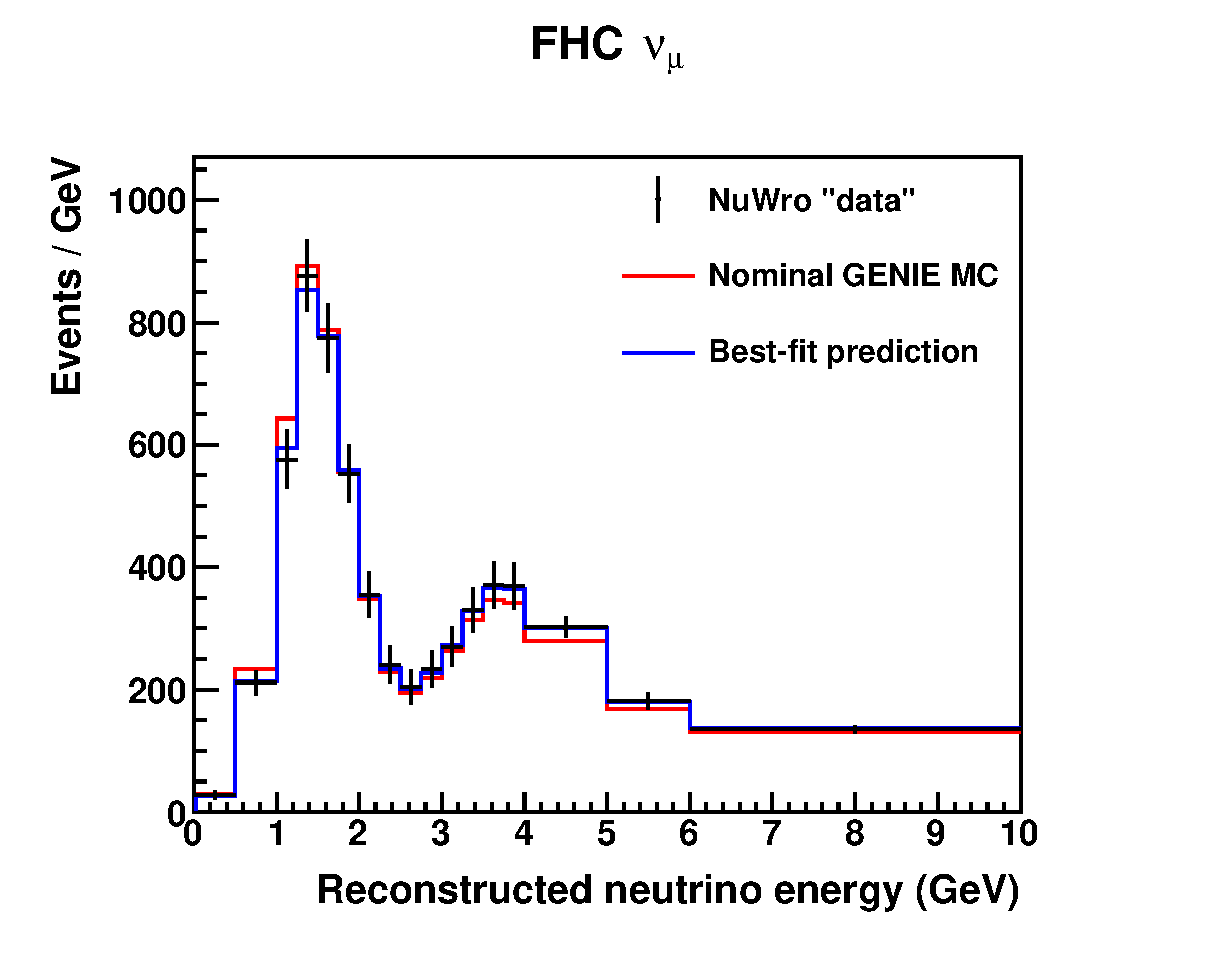
\includegraphics[width=0.45\columnwidth]{graphics/bf_dcp0_NumuFhc.eps}
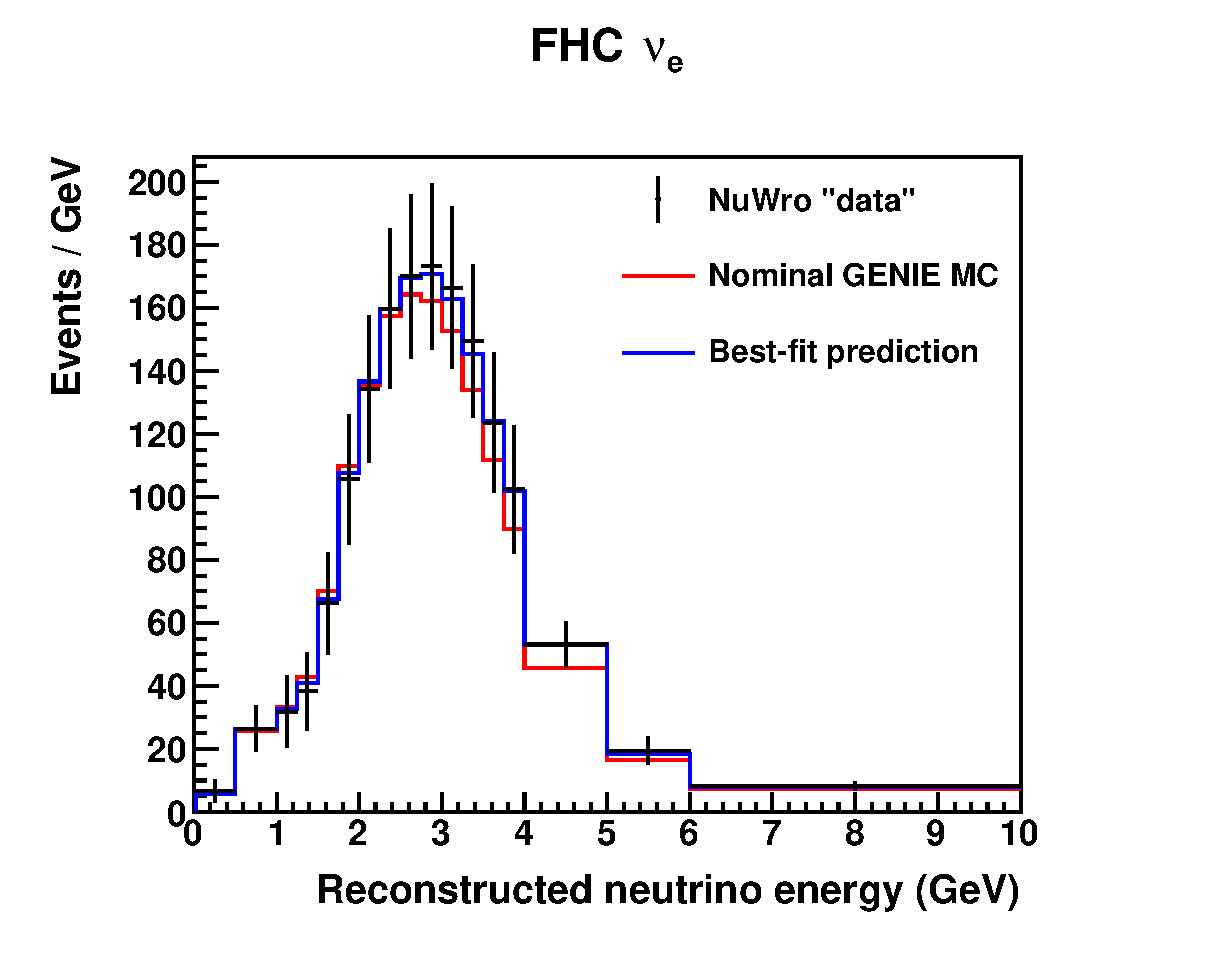
\includegraphics[width=0.45\columnwidth]{graphics/bf_dcp0_NueFhc.eps} \\
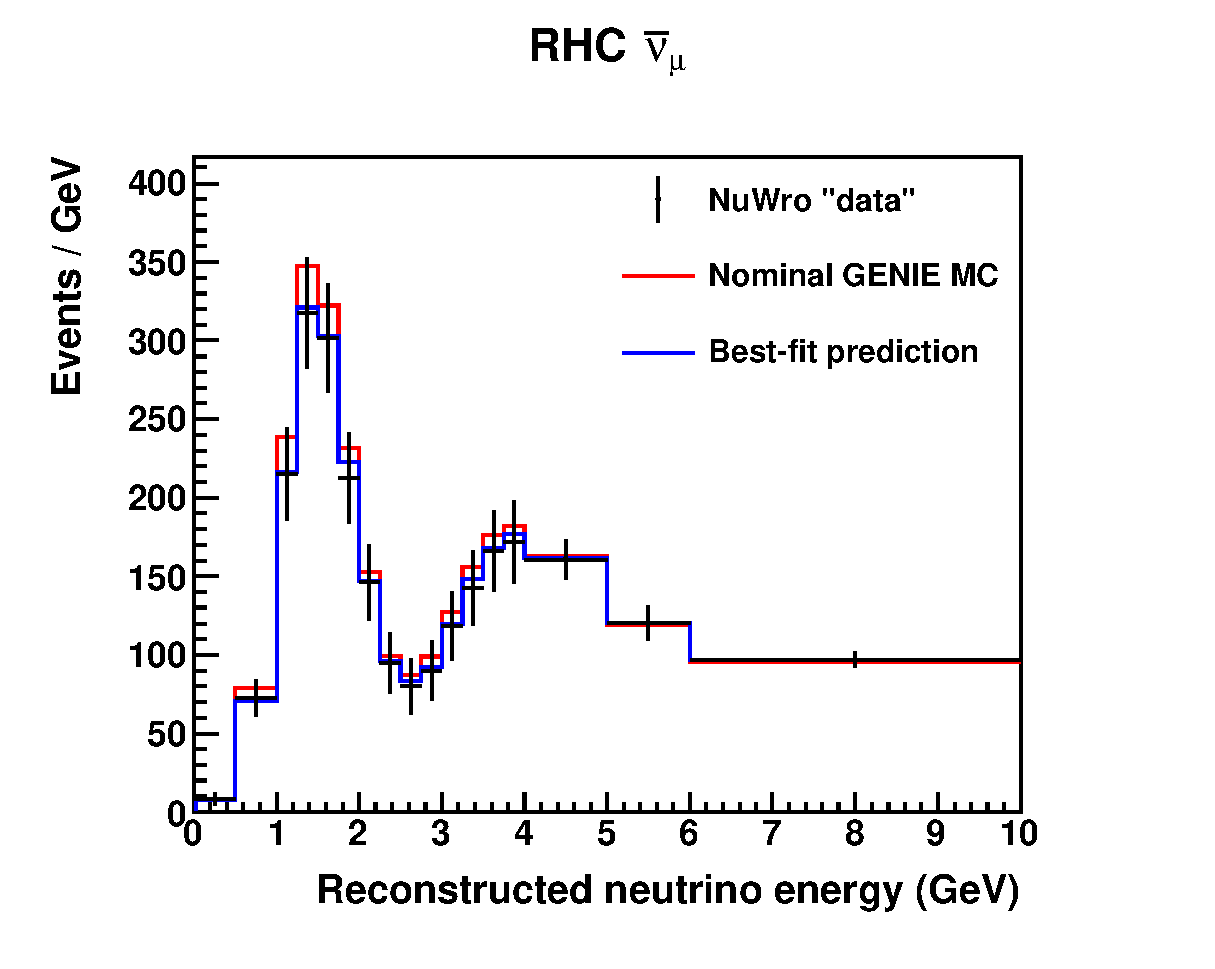
\includegraphics[width=0.45\columnwidth]{graphics/bf_dcp0_NumuRhc.eps}
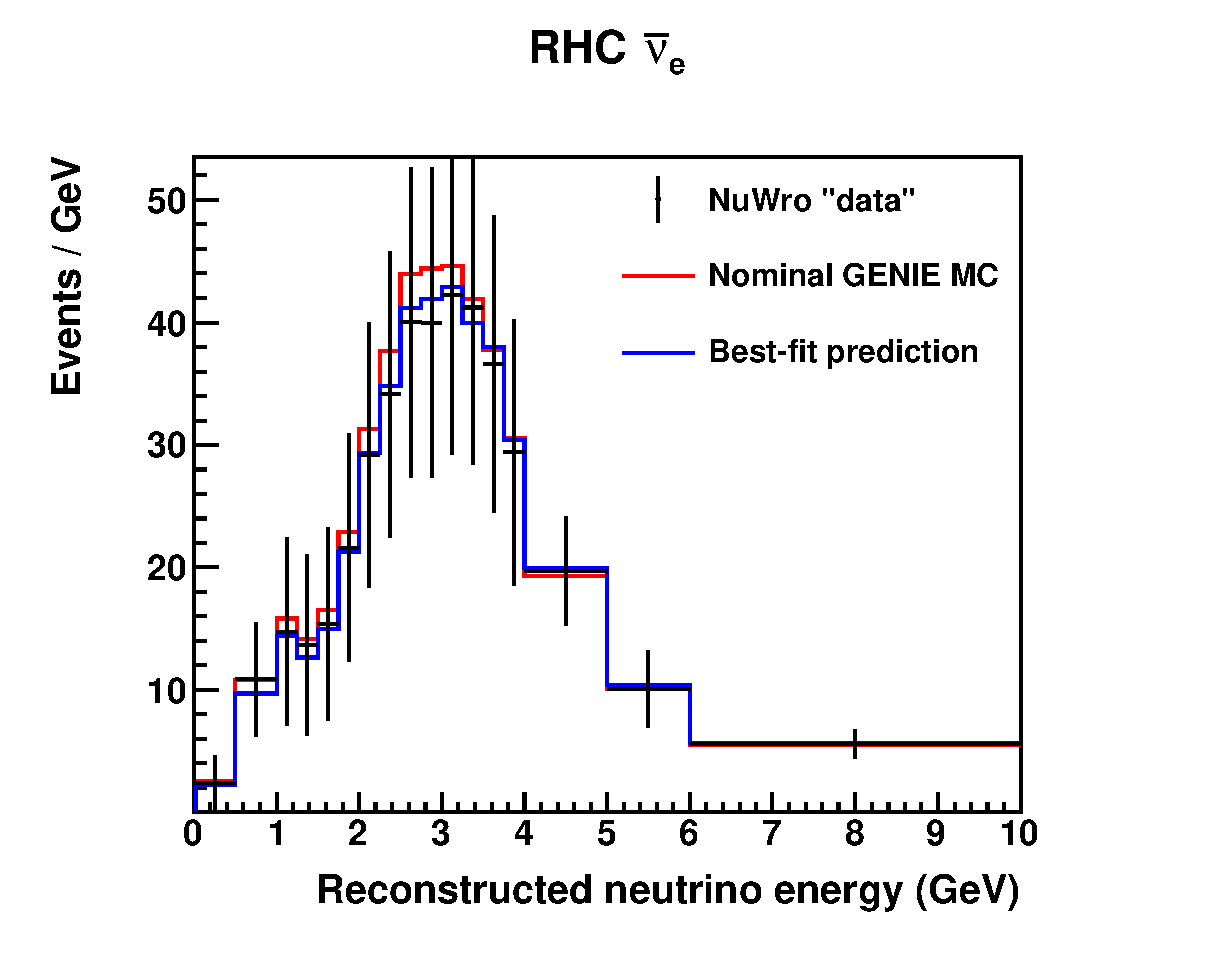
\includegraphics[width=0.45\columnwidth]{graphics/bf_dcp0_NueRhc.eps}
\caption{Far detector reconstructed spectra with the nominal GENIE MC (in red), compared to the NuWro mock data (black points), and the best-fit (blue), shown for the four FD samples, clockwise from top-left: }
\label{fig:nuwro_fdfit}
\end{figure}

This procedure is repeated for different true values of $\delta_{CP}$ with a flat prior. At each point, the bias in $\delta_{CP}$ is determined by comparing the best-fit value to the true value. The bias varies as a fuction of the true value of $\delta_{CP}$ as shown in Figure~\ref{fig:biasvsdcp}, and in fact for two points it happens to be zero. This is not surprising, and is due to the details of the NuWro-GENIE differences. The bias is correlated to biases in other oscillation parameters which also compensate for the differences between the two models. It would be inappropriate to conclude that for particular true values it is not necessary to consider out-of-model effects on $\delta_{CP}$. Instead, we evaluate the magnitude of this particular bias by taking the value that covers 68\% of the possible true values of $\delta_{CP}$. This can be interpreted as an additional uncertainty on the measured value of $\delta_{CP}$ in the case where there is no near detector to constrain the model sapce.


% Converting to CPV, skipping the gory details
The bias in $\delta_{CP}$ can be treated as an additional uncertainty due to the out-of-model effect. We estimate the impact of this additional uncertainty on the sensitivity to observe CP violation by assuming the bias is Gaussian and addint it in quadrature to the resolution on $\delta_{CP}$. With the Gaussian approximation on the additional contribution, this uncertainty on $\delta_{CP}$ is converted to a $\Delta \chi^{2}$ between the best-fit and the CP-conserving values $\delta_{CP} = 0,\pi$. This is done for each point in true $\delta_{CP}$, and we consider the sensitivity for maximal CP violation ($\delta_{CP} = -\pi/2$) and for at least 50\% of $\delta_{CP}$ values.
% The gory details
%First, for a given exposure and true value of $\delta_{CP}$, the resolution on $\delta_{CP}$ is determined. Second, the CP violation sensitivity based on the nominal in-model uncertainties by finding the $\Delta \chi^{2}$ between the best-fit and the CP-conserving values $\delta_{CP} = 0,\pi$, and taking the square root. Third, the out-of-model uncertainty is included by adding the bias in quadrature to the $\delta_{CP}$ resolution. Fourth, the $\delta_{CP}$ resolution is converted to a CP violation sensitivity both with and without the bias assuming that the uncertainty on $\delta_{CP}$ is Gaussian. The CP violation sensitivity is scaled by the ratio of this number with to without the bias added.

% No ND quick conclusion
Without any ND, the full bias must be taken as an uncertainty. This bias is not necessarily the worst-case scenario and there could be other out-of-model effects that lead to additional uncertainties. The FD alone is not sensitive to any plausible interaction modeling bias, as the statistics are insufficient to make precise measurements and the spectra are significantly impacted by oscillation parameters. The ``No ND'' band in Fig.~\ref{fig:nuwro_sens} shows the impact of one to three biases of this magnitude. The degredation in sensitivity clearly elminates the possibility of doing such a measurement without a near detector, so we do not further study this scenario with additional model variations.

\section{Constraining out-of-model effects with the ND}
\label{sec:ndconstraint}

The ND is used to constrain out-of-model effects by directly modifying the predicted FD spectra. By definition, the mock data cannot be matched by varying parameters in the reference model. Instead, the correction to the FD prediction is done directly based on quantities measured by the ND and extrapolated to the FD. This has a significant advantage in that it is possible to correct effects that are not known; it is not necessary to have a parameter that describes an observed discrepancy between data and simulation in order to extrapolate a correction to the FD. However, the process of extrapolation is inherently imperfect because cross sections depend on neutrino energy, and the neutrino fluxes at the ND and FD are different (mainly due to oscillations, but also due to the difference in solid angle of the ND and FD). Even if the ND is perfect, a model is required to relate a measurement in the ND flux to a prediction in the FD flux. 

The extrapolation can be done as a function of any quantity that can be measured in the ND. For this study, we define two quantities that are related to the energy and three-momentum transfer to the nuclear system, which we call the visible energy $E_{vis}$ and visible three-momentum transfer $p_{vis}$. In terms of truth quantities, the visible energy is 

\begin{equation}
E_{vis} = T_{p} + E_{\pi}
\end{equation}

\noindent
where $E_{\pi}$ is the total energy of all final-state pions, and $T_{p}$ is the kinetic energy of all final-state protons. Modulo binding energy, this is equivalent to the true energy transfer $q_{0}$ except that it excludes the energy transfered to neutrons, which are generally not observed. The visible momentum transfer is

\begin{equation}
\begin{split}
Q^{2} & = 2 E_{\nu} (E_{lep} - p_{lep} \cos \theta_{lep}) - m_{lep}^{2} \\
p_{vis} & = \sqrt{Q^{2} + E_{vis}^{2}}
\end{split}
\end{equation}

\noindent
where $E_{lep}$, $p_{lep}$, $m_{lep}$, and $\theta_{lep}$ are the total energy, three-momentum, mass, and angle with respect to the neutrino of the final-state lepton, and $E_{\nu}$ is the neutrino energy. These quantities are chosen because they describe the kinematics of the neutrino interaction, because different interaction topologies live in different regions of this space, and because the near detector can in principle measure it well.

Weights are determined by taking the ratio of the observed event rate as a function of $E_{vis}$ and $p_{vis}$ in the mock data to the reference model. This can be done either for an inclusive sample at the near detector, or separately for different interaction channels. The weights are then applied to the far detector predictions as a function of true $E_{vis}$ and $p_{vis}$. The result is that the corrected reference model more closely matches the mock data because differences in the models have been captured by the ND. The resulting bias to oscillation parameters is reduced or eliminated, depending on the quality of the ND reconstruction.

\subsection{Reconstruction in ND-LAr+TMS}

A parameterized reconstruction is applied to simulated events in ND-LAr. The muon energy is measured by range in LAr when it stops in the ND-LAr active volume. Exiting muons are measured in the downstream spectrometer. Events with muons that exit ND-LAr and do not enter the spectrometer are rejected. The hadronic energy is measured calorimetrically by adding all of the visible energy deposits in ND-LAr that are not associated with the muon. The reconstructed neutrino energy is the sum of the muon and hadronic energy components. The reconstructed $E_{vis} = E_{had}$; $p_{vis}$ is reconstructed by measuring the lepton kinematics and incorporating the hadronic energy estimate into the neutrino energy. 

Charged-current events are separated into exlusive interaction channels based on the number and charge of pions: $0 \pi$, $1 \pi^{\pm}$, $1 \pi^{0}$, $2 \pi$, $\ge 3 \pi$. Charged pions are identified based on the energy deposit at the end of the track. Hadron tracks which deposit more than 10 MeV in the last 1 cm of the track, or which deposit at least 5 MeV/cm in the first 3 cm are classified as protons. Hadron tracks with less than 10 MeV in the last 1 cm are classified as charge pions; the charge cannot be determined in ND-LAr so positive and negative pions are grouped together. Neutral pions are assumed to be reconstructed when both photons deposit at least 20 MeV in the detector.

The exclusive reconstruction in ND-LAr is excellent when all hadrons are above threshold ($\sim 1.5$~cm track length, about 50 MeV for protons), and when hadrons range out in the LAr volume without interacting hadronically. Particle indentification on very short tracks is typically impossible, because the charge deposits very near the vertex often contain contributions from several particles, which complicates the dE/dx measurement of any one track. Interacting hadrons are also challenging to identify, because both protons and charged pions can induce similar hadronic showers. The exception is when the track is sufficiently long and heavily ionizing that it can be identified as a proton despite the shower. However, ionization fluctuations lead to ambiguities. Figure~\ref{fig:lar_matrices} shows the ambiguity matrix for the multiplicity of charged hadrons (protons and charged pions), and the confusion matrix for different exclusive final states. The feed-down in the hadron multiplicities is due almost entirely to sub-threshold protons; imposing a threshold eliminates this feed-down.

\begin{figure}[h]
\centering
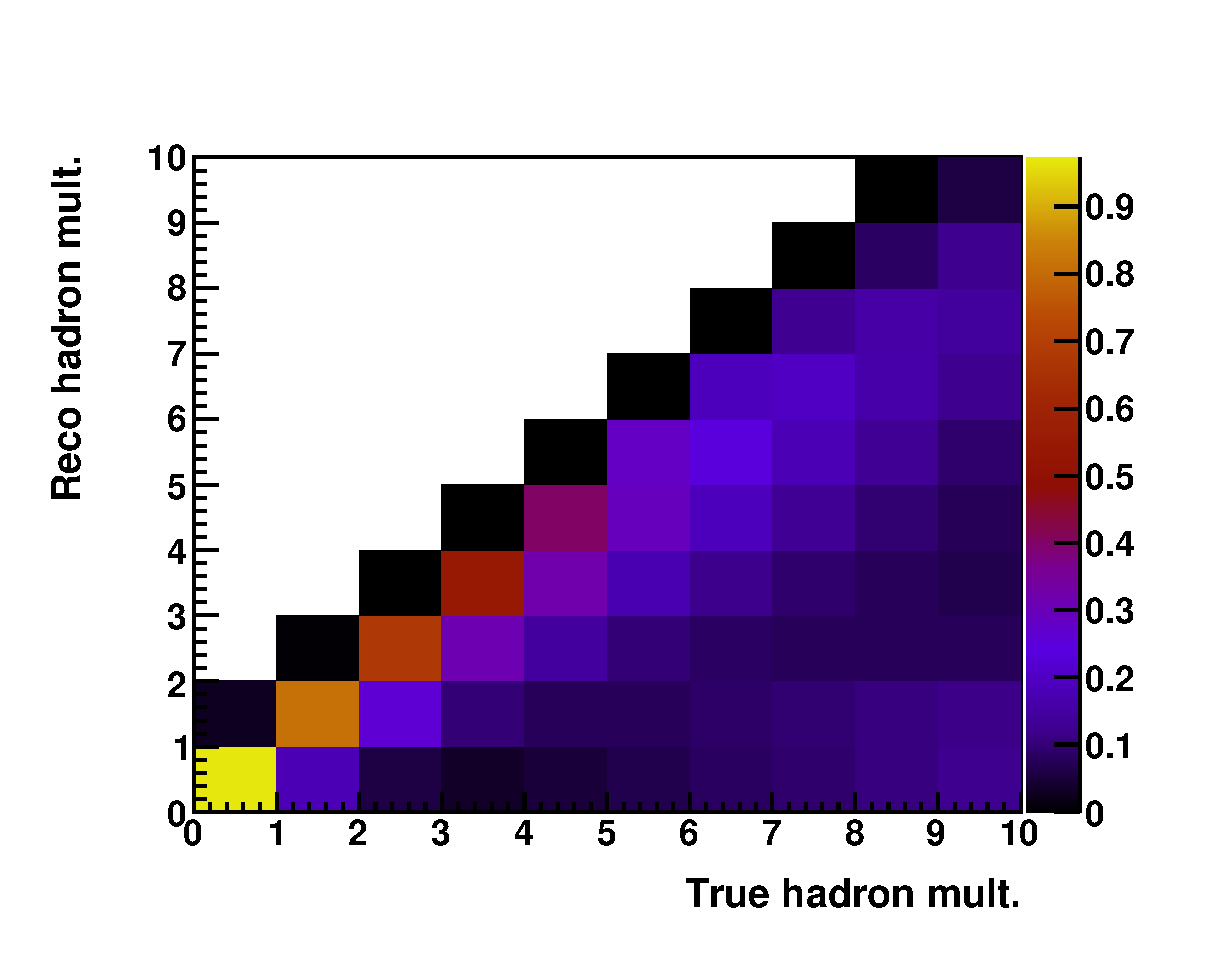
\includegraphics[width=0.45\columnwidth]{graphics/hadMult_matrix_colNorm.eps}
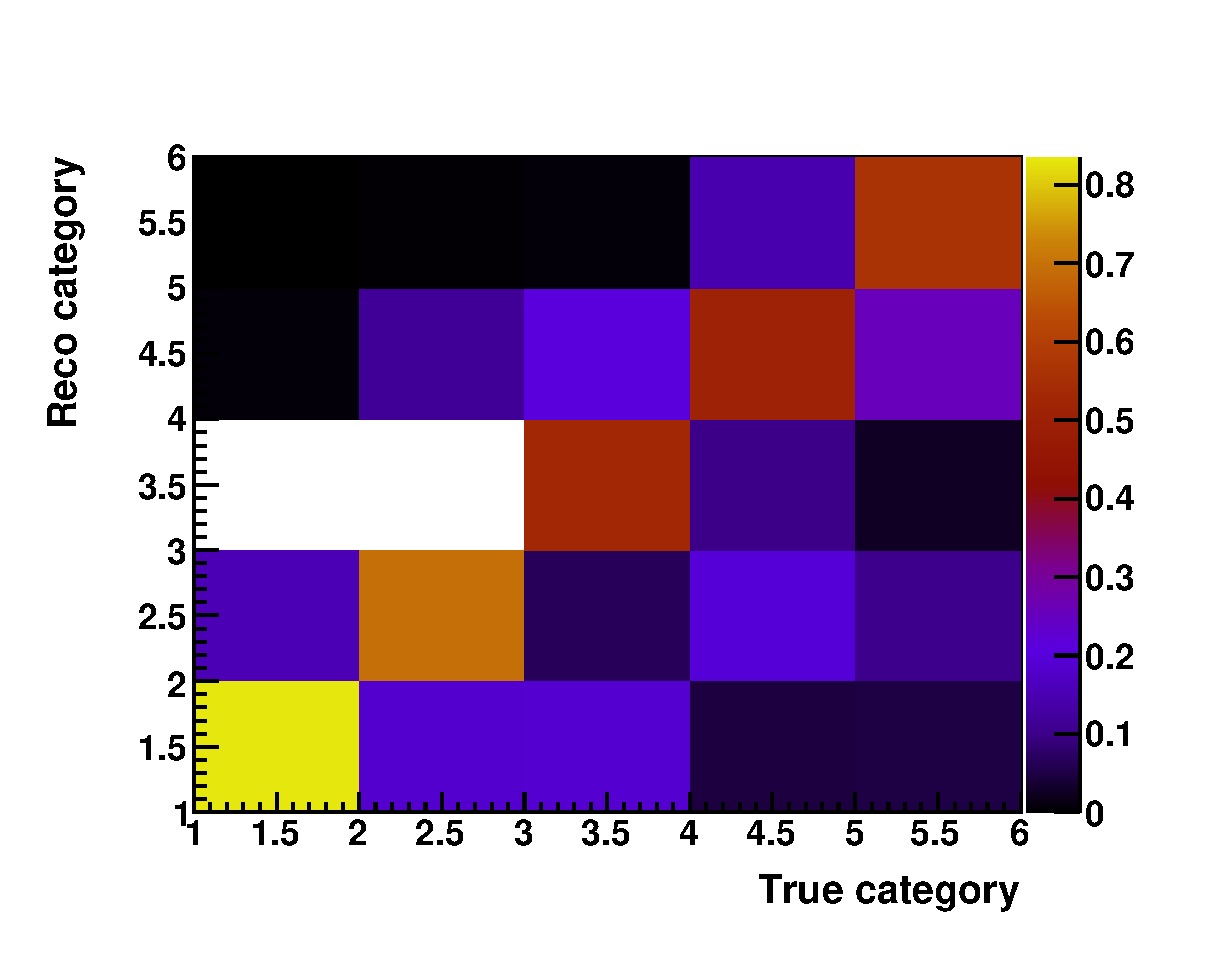
\includegraphics[width=0.45\columnwidth]{graphics/confusion_matrix_colNorm.eps}
\caption{The confusion matrix for the multiplicity of charged hadrons (left), showing significant feed-down from high true multiplicity to lower reconstructed multiplicity (below the diagonal) due to particles that are below detection threshold. The confusion matrix for exclusive interaction channels (right), where 1 = CC$0\pi$, 2 = CC$1\pi^{\pm}$, 3 = CC1$\pi^{0}$, 4 = CC$2\pi$ of any charge, and 5 = CC with at least three pions.}
\label{fig:lar_matrices}
\end{figure}

The reconstruction of $E_{vis}$ is excellent for events without neutrons. Neutrons in the kinetic energy range of 50-300 MeV deposit $\sim 20$\% on average of their total kinetic energy in the detector in the form of knock-out protons from neutron-argon interactions, with a large spread. This leads to a mismeasurement of $E_{vis}$, and there is not another quantity that tracks the physics of the hadronic side of the neutrino interaction that is well measured because the inability to see neutrons is fundamental. Simply excluding them from the LAr estimator is also not perfect, because they indeed deposit nontrivial amounts of energy in the detector. Even if we could identify neutron energy deposits in LAr and subtract them, this would still be problematic because neutrons are often produced in hadronic showers of charged particles. This is a fundamental limitation of ND-LAr that is due to the relatively high density of the detector medium. It is not expected that any algorithmic improvement will be capable of identifying neutrons that are produced directly in the neutrino interaction and also differentiating those neutrons from neutrons produced inside the detector.

The ratio of NuWro to GENIE is shown as a function of $Q^{2}$ in the left panel of Figure~\ref{fig:lar_ratios}. The lines show the ratio as a function of true $Q^{2}$ for all CC events and also broken up into several exclusive channels based on truth. The points show the same quantity in reconstruction, where the division into exclusive channels is also based on reconstruction. Generally, the true and reco ratios agree better at low momentum transfer. The reconstruction worsens as the momentum transfer increases and is especially poor for final states with multiple pions. The ratio of NuWro to GENIE for all CC events is show as a function of the reconstructed energy and momentum transfer as defined above in the right panel of Figure~\ref{fig:lar_ratios}. The same general feature can be observed; NuWro predicts fewer events at very low momentum transfer and an excess at high momentum transfer.

\begin{figure}[h]
\centering
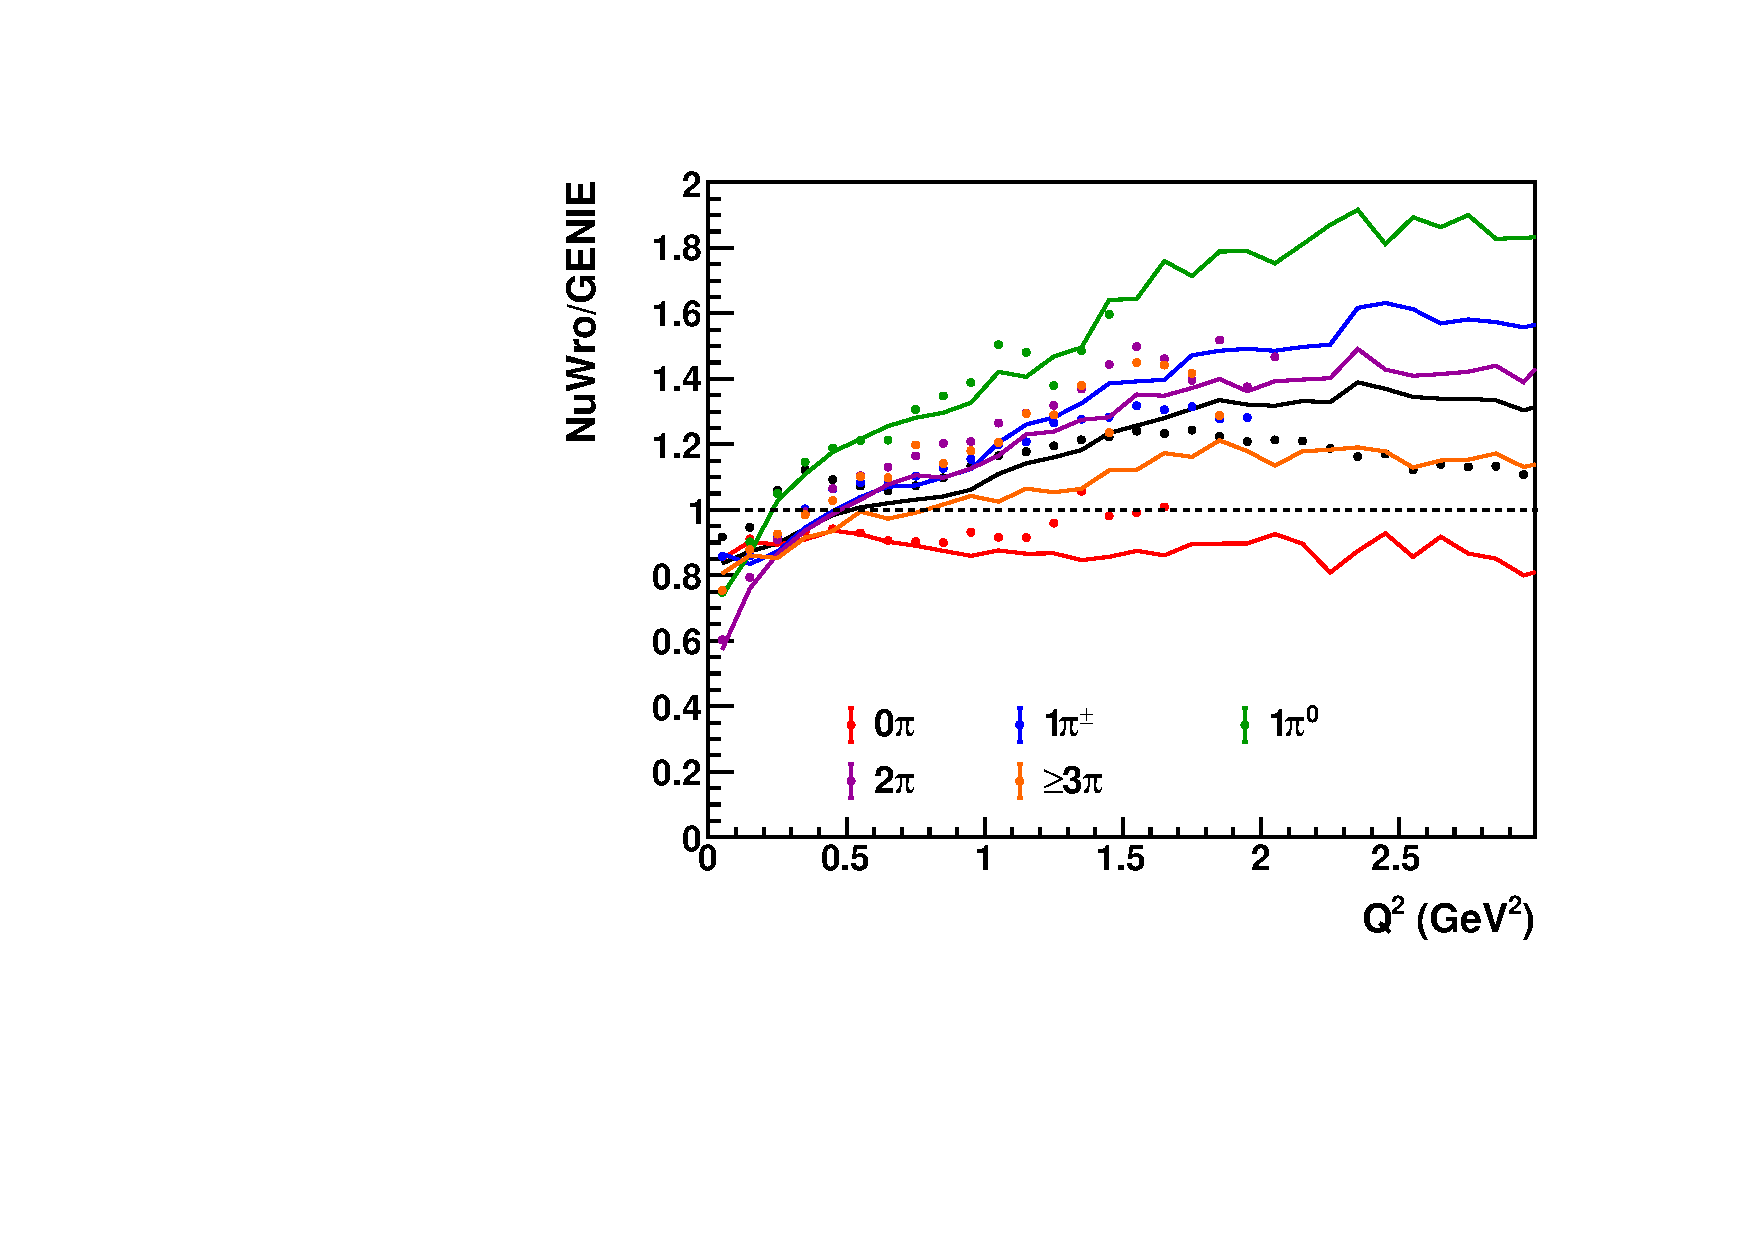
\includegraphics[width=0.45\columnwidth]{graphics/LAr_TrueRecoRatios_Q2.pdf}
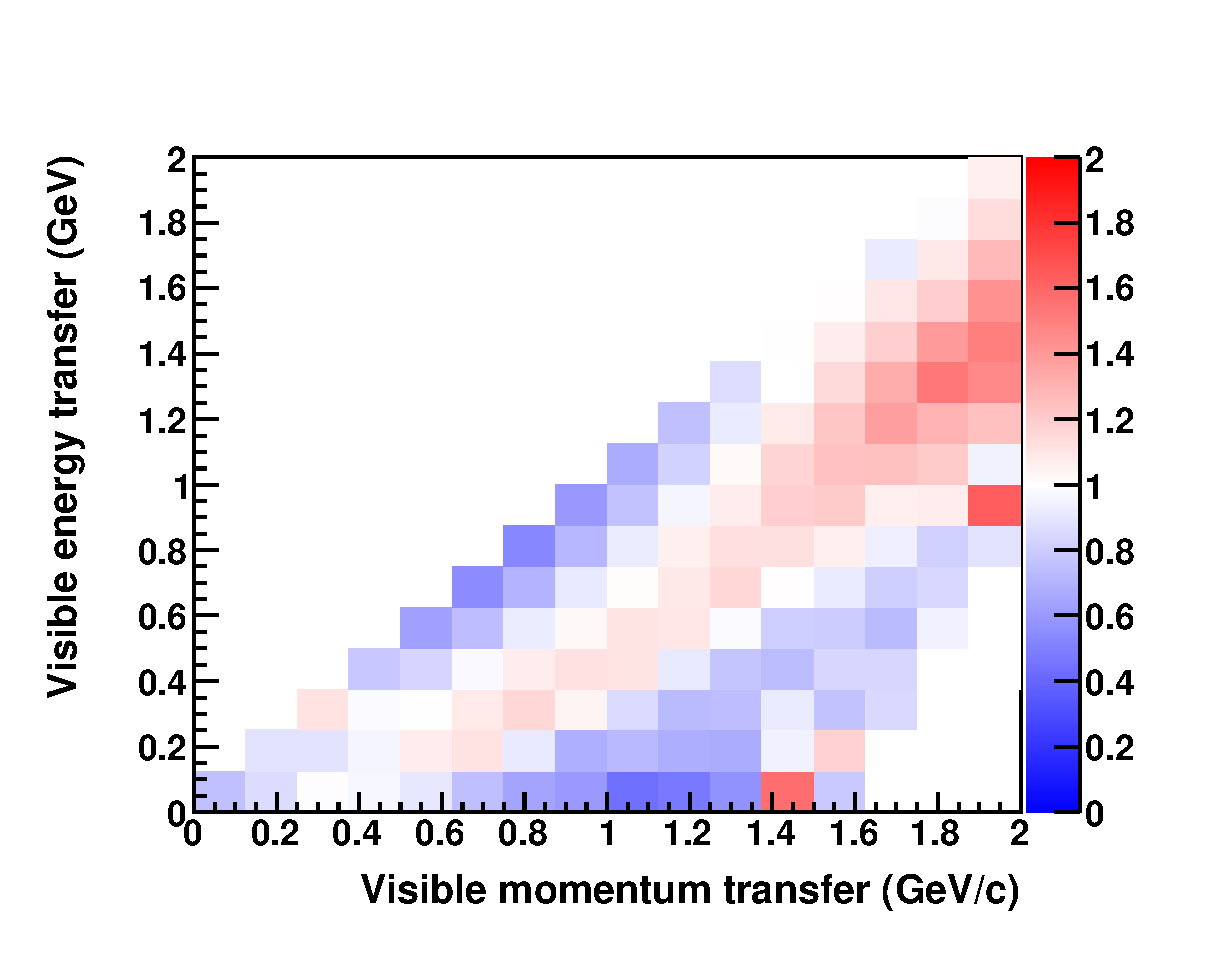
\includegraphics[width=0.45\columnwidth]{graphics/ratio_q0q3_all.eps}
\caption{The true and reconstructed ratios between NuWro and GENIE as a function of $Q^{2}$ (left), and the reconstructed ratio as a function of $p_{vis}$ and $E_{vis}$ (right).}
\label{fig:lar_ratios}
\end{figure}

Weights derived from the reconstructed ND spectra are applied to the FD predictions as a function of true $p_{vis}-E_{vis}$. When the LAr-derived weights are applied, the discrepancy shown in Fig.~\ref{fig:nuwro_fdfit} is reduced. For the ND-LAr reconstruction, very little is gained by separating the sample into exclusive channels. This is primarily because the different final states shown in the left panel of Fig.~\ref{fig:lar_ratios} populate different regions of the $p_{vis}-E_{vis}$ space. The smearing between the event categories is large, and so separating by essentially dividing the $p_{vis}-E_{vis}$ space is not significantly different from dividing it based on pion counting.

\subsection{Reconstruction with ND-GAr}

Neutrino interactions inside the ND-GAr fiducial volume can be reconstructed with higher fidelity due to the very low momentum threshold, the absence of hadron re-interactions, the more uniform acceptance as a function of energy and angle, and the sign selection capability for any charged track. Charged particle momenta are reconstructed by curvature, and particle identification combines the dE/ds in the gas, the energy deposited in the surrounding calorimeter, and the momentum measurement. There is essentially no pion/proton confusion for momenta below 1 GeV/c, so the confusion between different interaction channels is at the few percent level, an order of magnitude smaller than the 20-30\% seen in ND-LAr. This is shown for FHC and RHC in Figure~\ref{fig:gar_matrices}.

\begin{figure}[h]
\centering
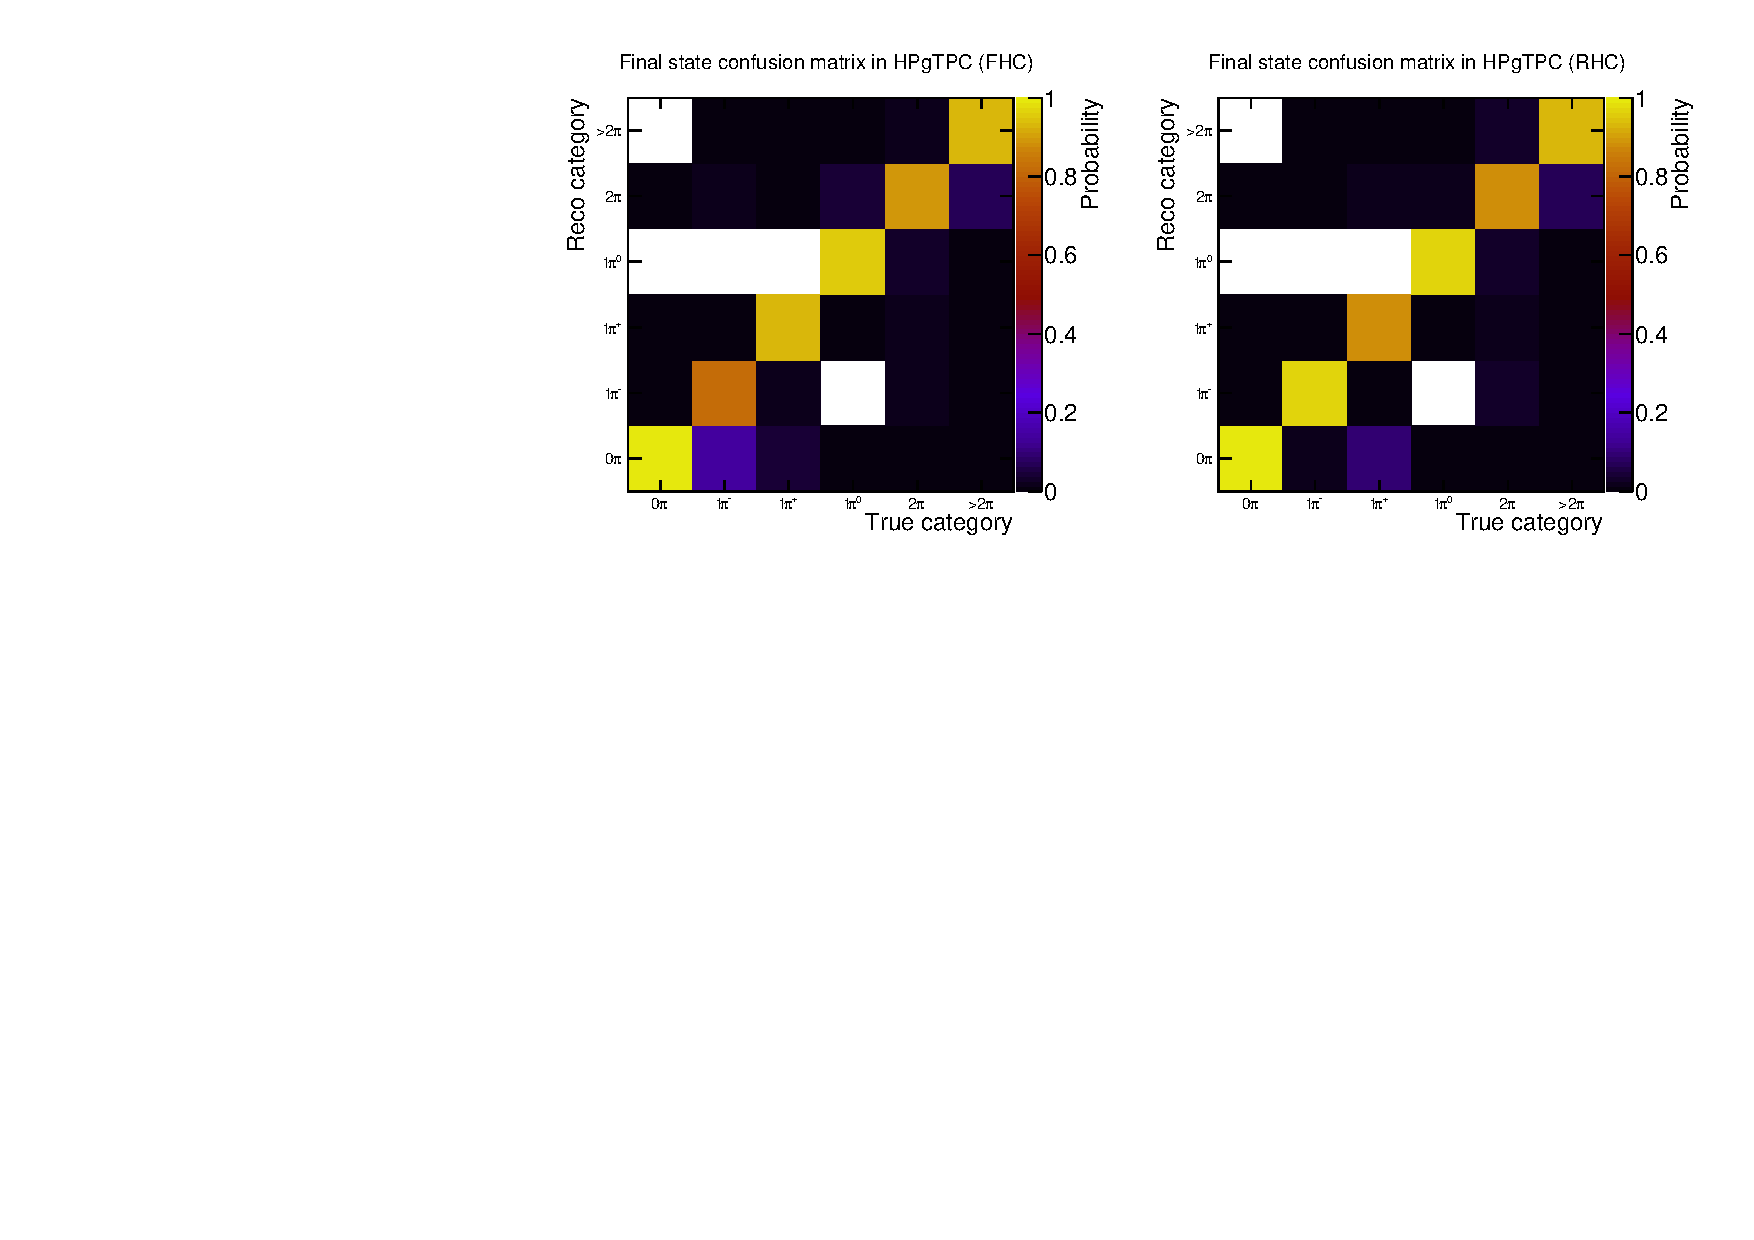
\includegraphics[width=0.9\columnwidth]{graphics/PiStudyConfusionMatrixBoth.pdf}
\caption{Confusion matrices between reconstructed and true event topologies in ND-GAr. The confusion is much smaller than in ND-LAr due to the absence of hadron re-interactions, and the superior pion/proton identification using dE/dx and the measured momentum of the hadron.}
\label{fig:gar_matrices}
\end{figure}

The reconstruction of $E_{vis}$ and $p_{vis}$ is also superior in ND-GAr. This is primarily due to the ease of excluding primary neutrons from the hadronic energy because they do not interact in the GAr volume. Also, the calorimetric hadronic energy measurement in LAr typically misses the masses of charged pions; in ND-GAr, these pions are easily identified and their masses are added. The result is that the weights derived from ND-GAr better reproduce the FD spectra and result in a much smaller bias to the measurement of oscillation parameters including $\delta_{CP}$.

\subsection{Oscillation fits with the reweighted prediction}

The oscillation fit is repeated with the reweighted reference MC replacing the default GENIE. The reweighting reduces the bias in $\delta_{CP}$ significantly. Because of the flux differences, it is not possible to completely eliminate the bias, but a good constraint should yield a bias that is much smaller than the resolution on $\delta_{CP}$ due to in-model uncertainties. The ultimate resolution on $\delta_{CP}$ is $\sim 7^{\circ}$ in the case where CP is conserved and $\sim 15^{\circ}$ in the maximally CP violating case, as shown in Fig.~\ref{fig:longterm_sensitivity}. 

The bias in the oscillation fit including the reweighting based on the Day 1 ND and based on the reference ND is shown in Figure~\ref{fig:biasresults}. The shape of the bias as a function of true $\delta_{CP}$ depends on the details of the mock data. We take the magnitude of the bias as the value that covers 68\% of the true $\delta_{CP}$ space. This is $16.2^{\circ}$ in the case of no ND constraint, reduced to $8.6^{\circ}$ in the case of the Day 1 ND, and less than $4^{\circ}$ when the ND-GAr data is included.

\begin{figure}[h]
\centering
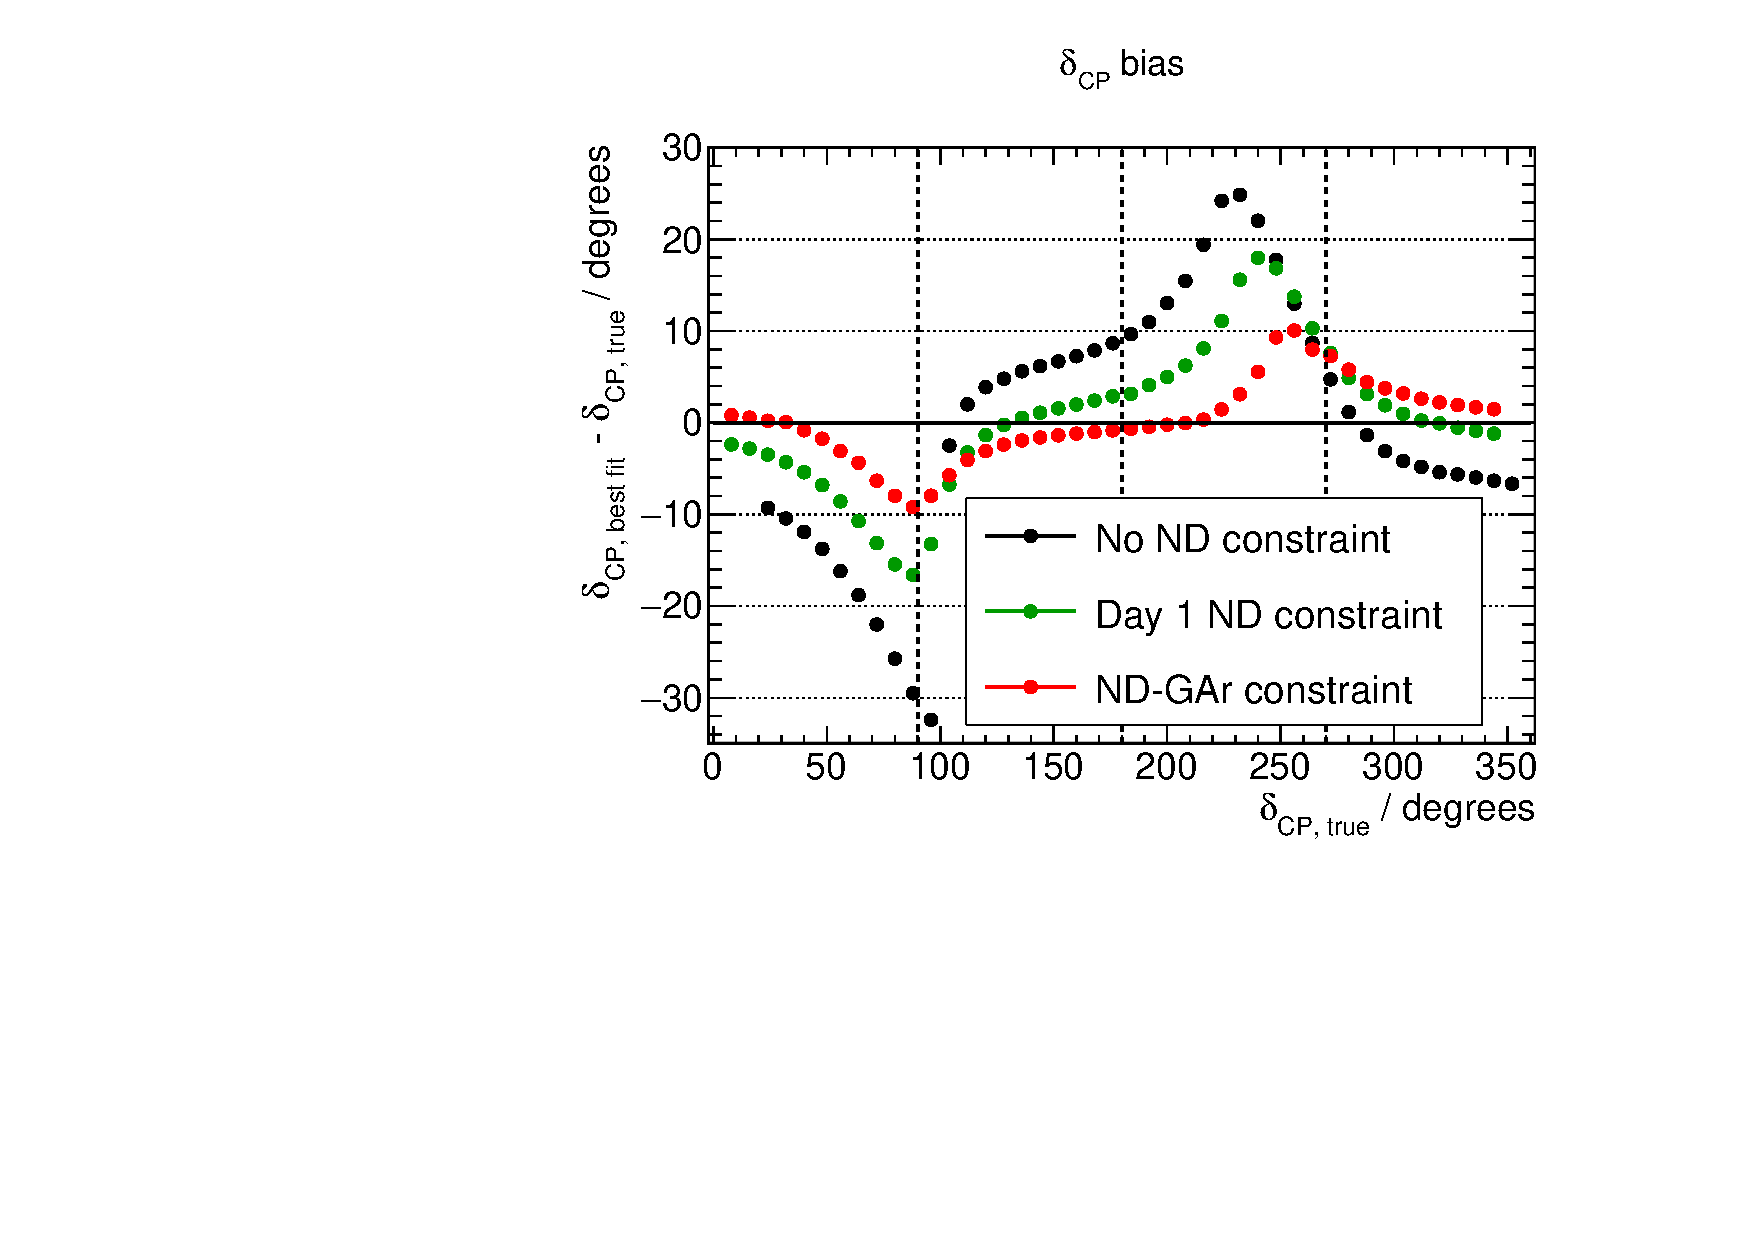
\includegraphics[width=0.9\columnwidth]{graphics/PiStudyBiasWithGAr.pdf}
\caption{The bias in $\delta_{CP}$ resulting from a FD fit to the NuWro mock data with no ND constraint, with the Day 1 ND constraint, and with the reference ND constraint using ND-GAr.}
\label{fig:biasresults}
\end{figure}

The bias is incorporated into the CP sensitivity using the procedure described in Section~\ref{sec:mockdata}. The result is the CP violation sensitivities including the out-of-model uncertainty shown in Figure~\ref{fig:nuwro_sens}. The maximal CP violation case is evaluated with $\delta_{CP} = -\pi/2$.

\section{Conclusions}
\label{sec:conclusions}

This LAr reconstruction significantly reduces the observed bias in oscillation parameters including $\delta_{CP}$, but does not entirely eliminate it. The bias in $\delta_{CP}$ for 68\% of true values is 8.6$^{\circ}$, reduced by nearly a factor of two from the bias without any reweighting of 16.2$^{\circ}$. As shown in Figure~\ref{fig:nuwro_sens}, it does not significantly worsen the sensitivity to maximal CP violation over timescales of several years. This is because the $\delta_{CP}$ resolution for maximal CP violation is 30-60$^{\circ}$ during this early data taking period, which can be seen in Fig.~\ref{fig:longterm_sensitivity}. The unconstrained bias of 16.2$^{\circ}$ is specific to this particular selection of mock data; it is conceivable that nature could be even worse. However, the residual bias including the constraint from ND-LAr + TMS is less sensitive to the details of the mock data. It is governed mainly by the resolutions on ND-LAr + TMS, especially for hadronic energy, and also to flux differences between ND and FD and their impact on the cross section. The latter effect can be studied in detail with off-axis data and PRISM, even in the LAr + TMS configuration, and its impact can be controlled.

Furthermore, there are several plausible analysis improvements that could somewhat improve the LAr constraint. In this study, we extrapolate to the FD in terms of true quantities, which are imperfectly measured in ND-LAr and TMS. We might instead apply the weights at the FD in terms of reconstructed quantities, and leverage similarities in the hadronic energy reconstruction in different interaction channels between ND and FD. We do not presently have a detailed understanding of how well this will work given the differences between the readout technology in the two detectors, but it will almost certainly be an improvement over what is assumed here, which is essentially zero correlation between the reconstruction at ND and FD. It may also be possible to directly incorporate reconstructed neutrino energy into the constraint.

Some more conclusions probably.

















\end{document}

